\documentclass[titlepage,landscape]{seminar}
\usepackage{url}
\usepackage{graphicx}
\usepackage[pdftex]{color}
\usepackage{hyperref}
\usepackage{epstopdf}
\usepackage{slides}

\newcommand{\frack}{\frac{1}{k}}
\newcommand{\quarter}{\frac{1}{4}}

\begin{document}

\myslide{
\heading{{\it Melanopus oregonensis}}
\begin{center}
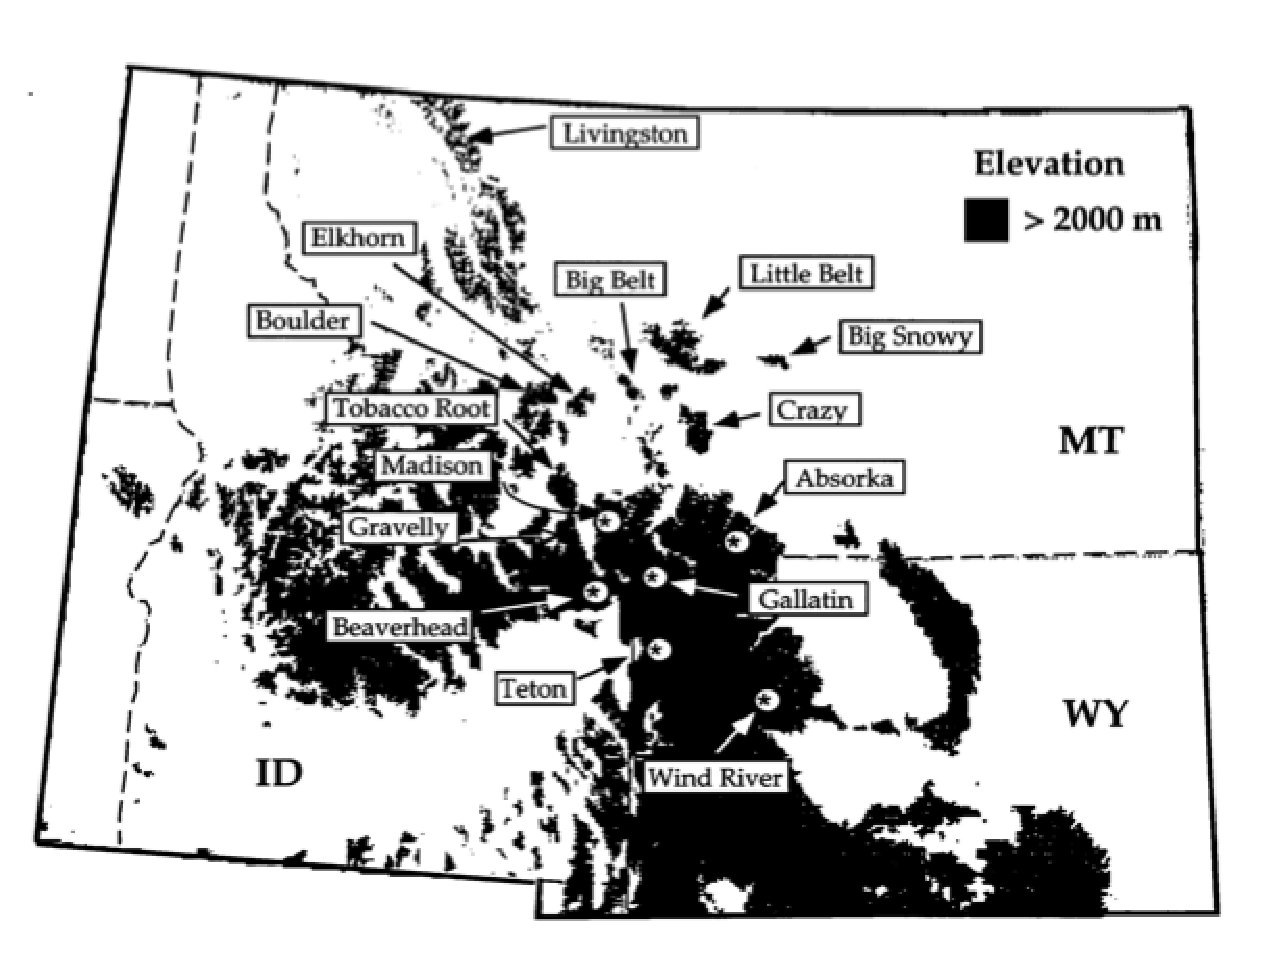
\includegraphics[height=0.9\textheight]{sky-islands.eps}
\end{center}
}

\myslide{
\heading{{\it Melanopus oregonensis}}
\begin{itemize}

\item {\bf Widespread ancestor}: The existing populations might represent
  independently derived remnants of a single, widespread
  population. In this case all of the populations would be equally
  related to one another.

\item {\bf Multiple glacial refugia}: Populations that shared the same
  refugium will be closely related while those that were in different
  refugia will be distantly related.

\end{itemize}
}

\myslide{
\heading{{\it Melanopus oregonensis}}
\begin{center}
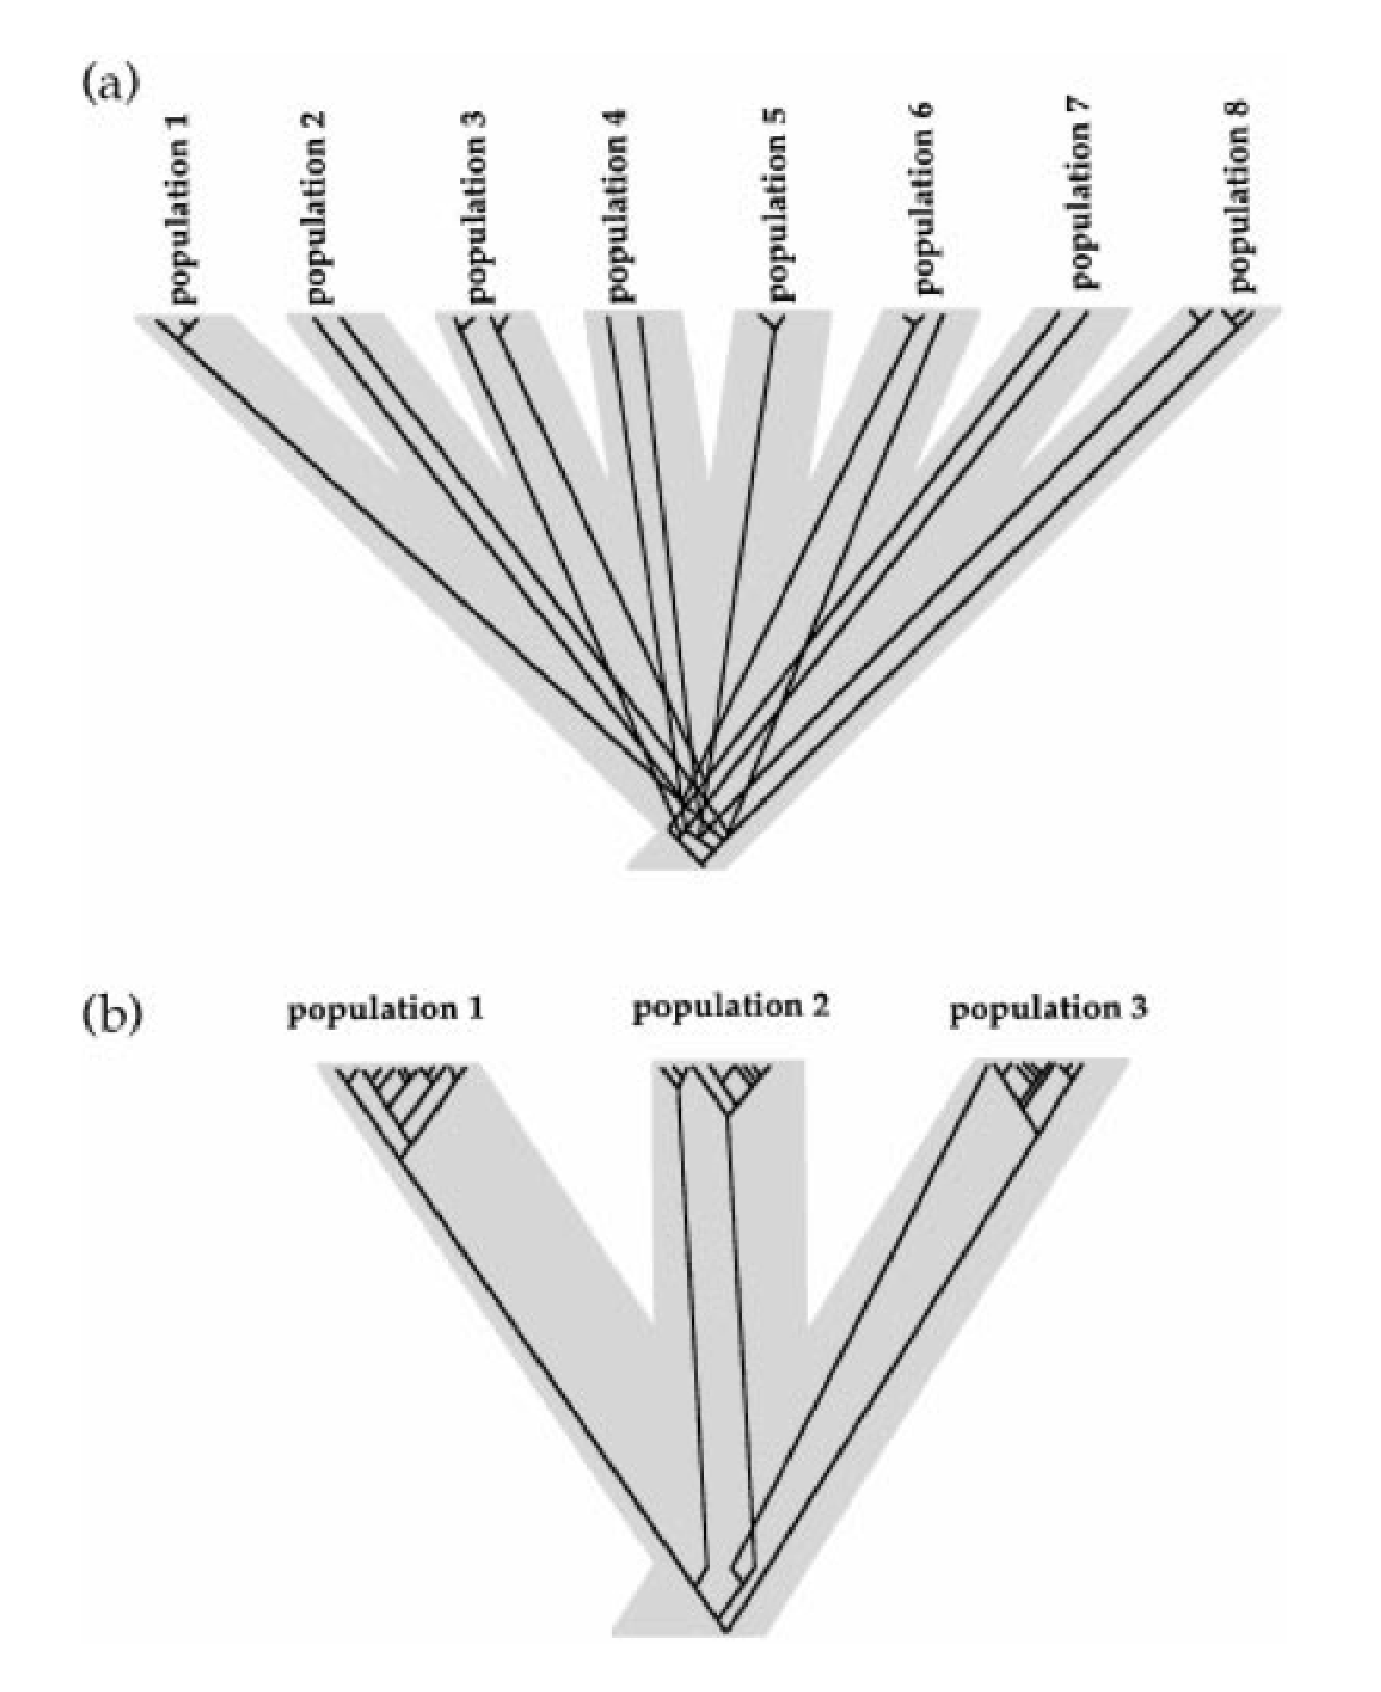
\includegraphics[height=6cm]{divergence-hypotheses.eps}
\end{center}
}

\myslide{
\heading{{\it Melanopus oregonensis}}
\begin{itemize}

\item Estimate the the phylogeny of the haplotypes in the sample. 

\item Estimate $s_{obs}$,  the minimum number of among-population  migration
  events necessary to account for where haplotypes are currently found
  given the inferred phylogeny.

\item Simulate a neutral coalescence process in which the populations
  are derived from a single, widespread ancestral population. 

\item Rearrange the data so that populations are grouped into separate
  refugia.

\item Estimate $s_{sim}$ from the rearranged data, and repeat this 100
  times for several different times since population splitting.

\end{itemize}
}

\myslide{
\heading{{\it Melanopus oregonensis}}
\begin{center}
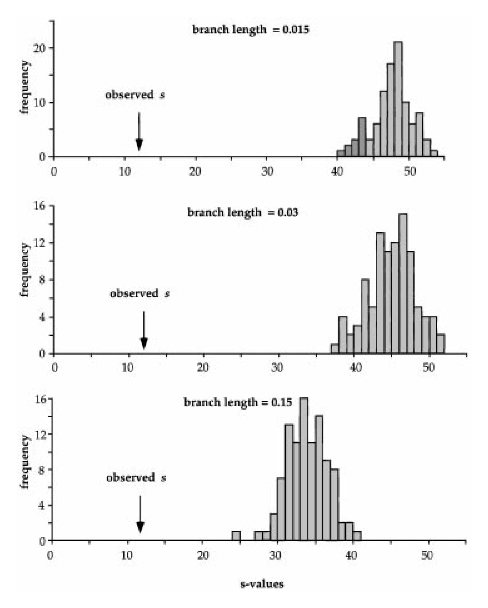
\includegraphics[height=0.9\textheight]{knowles-s-values.eps}
\end{center}
}

\myslide{
\heading{{\it Bufo marinus}}
\begin{center}
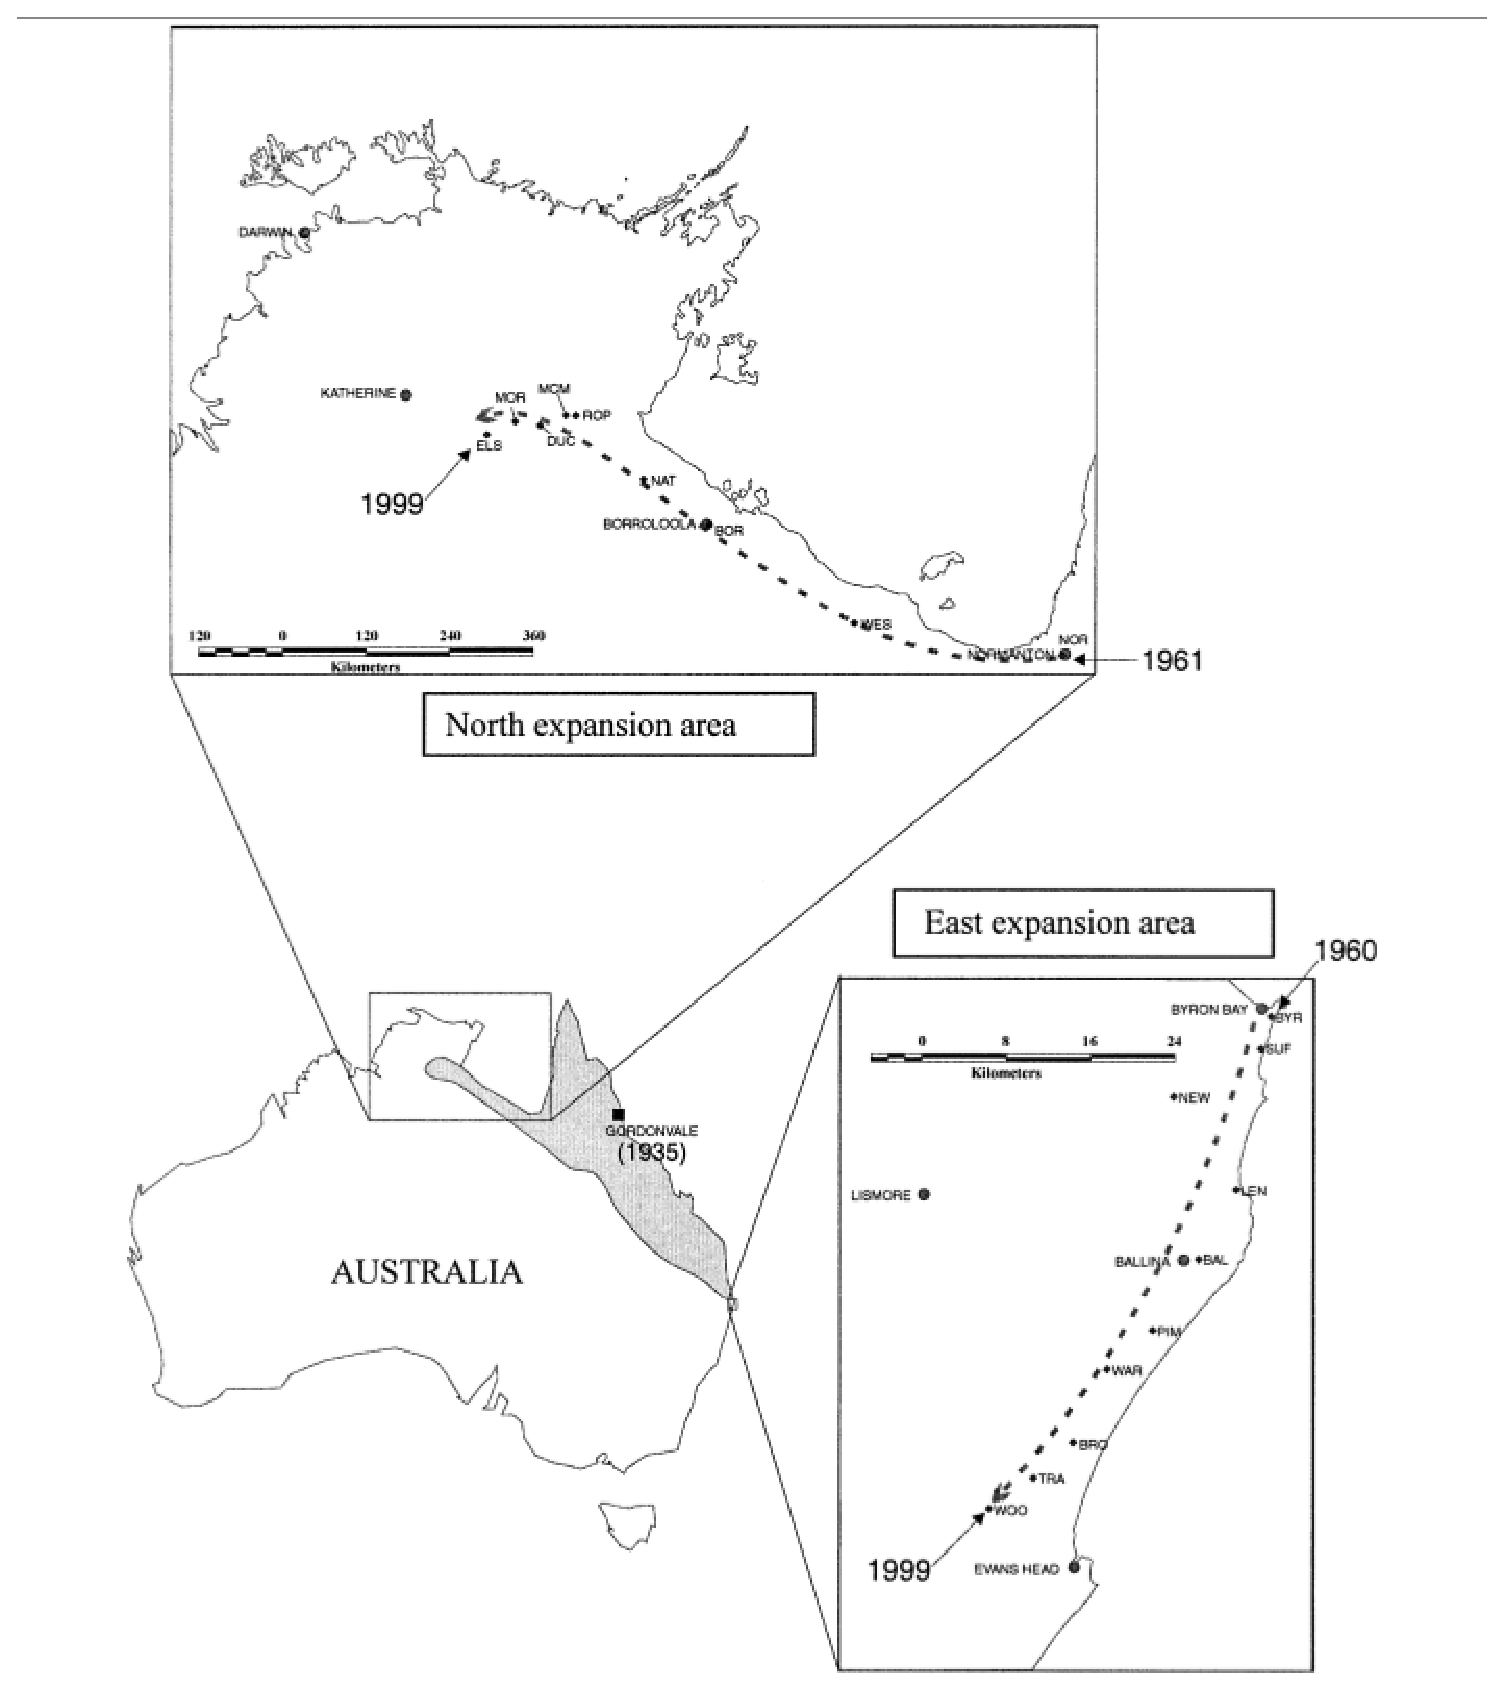
\includegraphics[width=0.8\textheight]{cane-toad-expansion.eps}
\end{center}
}

\myslide{
\heading{{\it Bufo marinus}}
\begin{enumerate}

\item Isolation by distance

\item Differential migration and founding

\item ``Island'' migration and founding

\item Stepwise migration and founding with founder events

\item Stepwise migration and founding without founder events

\end{enumerate}
}

\myslide{
\heading{Approximate Bayesian Computation (ABC)}
\[
\mbox{P}(X|\xi) = \mbox{likelihood of data, $X$, given parameters $\xi$}
\]
\vfill
\begin{enumerate}

\item Calculate ``appropriate'' summary statistics for your data set,
  $S$. 

\item Specify a prior distribution for the unknown parameters, $\xi$.

\item Pick $\xi'$ from the prior distribution and simulate data.

\item Calculate $S'$ from the simulated data.

\item Calculate the distance, $\delta$ between $S$ and $S'$.

\item If $\delta < \delta_{max}$, keep $S'$ and $\xi'$. Otherwise,
  discard them. 

\item Return to step 3 and repeat until you you have accepted a large
  number of pairs of $S'$ and $\xi'$.

\end{enumerate}
}

\myslide{
\heading{Approximate Bayesian Computation (ABC)}
\vfill
Fit the following regression:
\[
\xi_i = \alpha + S_i\beta + \epsilon 
\]
\vfill
``Predict'' $\xi$ for our observed data
\[
\xi = \alpha + S\beta + \epsilon 
\]
}

\myslide{
\heading{{\it Bufo marinus}}
\begin{center}
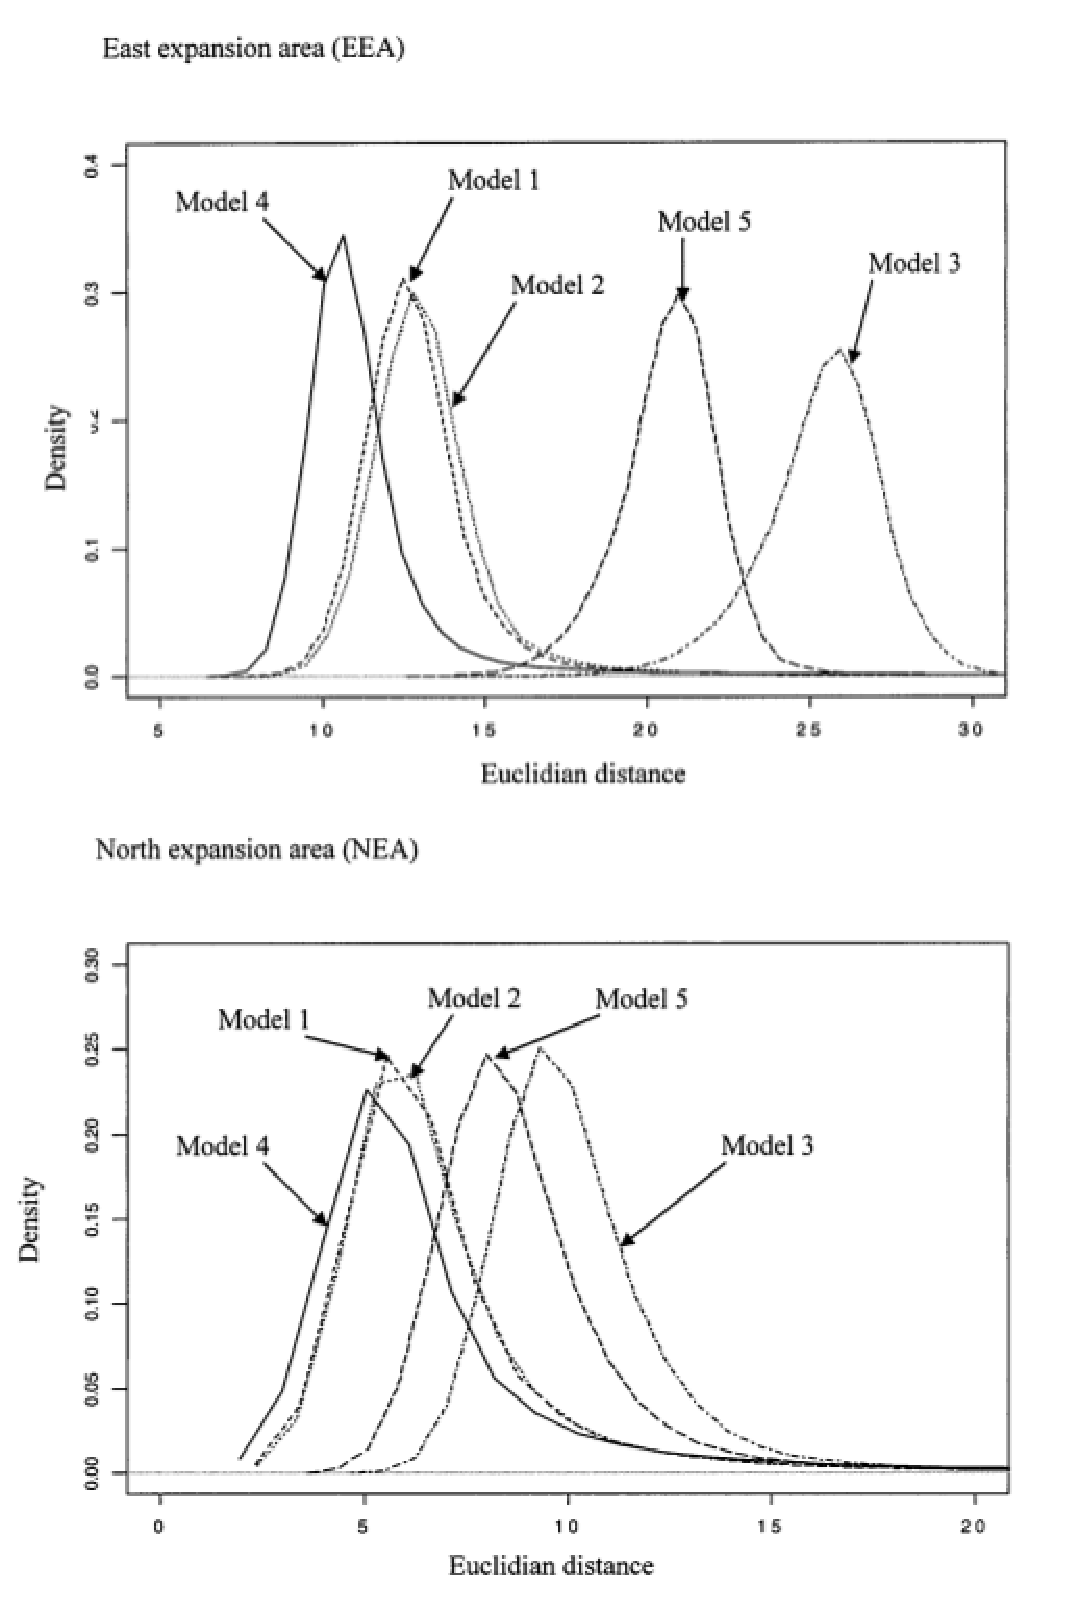
\includegraphics[height=0.9\textheight]{cane-toad-models.eps}
\end{center}
}

\myslide{
\heading{{\it Bufo marinus\/} (Model 4)}
\begin{center}
\begin{tabular}{ccr}
\hline\hline
Parameter & area & mean (5\%, 90\%) \\
\hline
$N_{e_s}$ & east & 744 (205, 1442) \\
         & north & 1685 (526, 2838) \\
$N_{e_f}$ & east & 78 (48, 118) \\
         & north & 311 (182, 448) \\
$F_R$    & east & 10.7 (2.4, 23.8) \\
         & north & 5.9 (1.6, 11.8) \\
$m$      & east & 0.014 ($6.0 \times 10^{-6}$, 0.064) \\
         & north & 0.117 ($1.4 \times 10^{-4}$, 0.664) \\
$N_{e_s}m$ & east & 4.7 (0.005, 19.9) \\
          & north & 188 (0.023, 883) \\
\hline
\end{tabular}
\end{center}
}

\myslide{
\heading{{\it Wyeomyia smithii\/} ({\it COI\/})}
\begin{center}
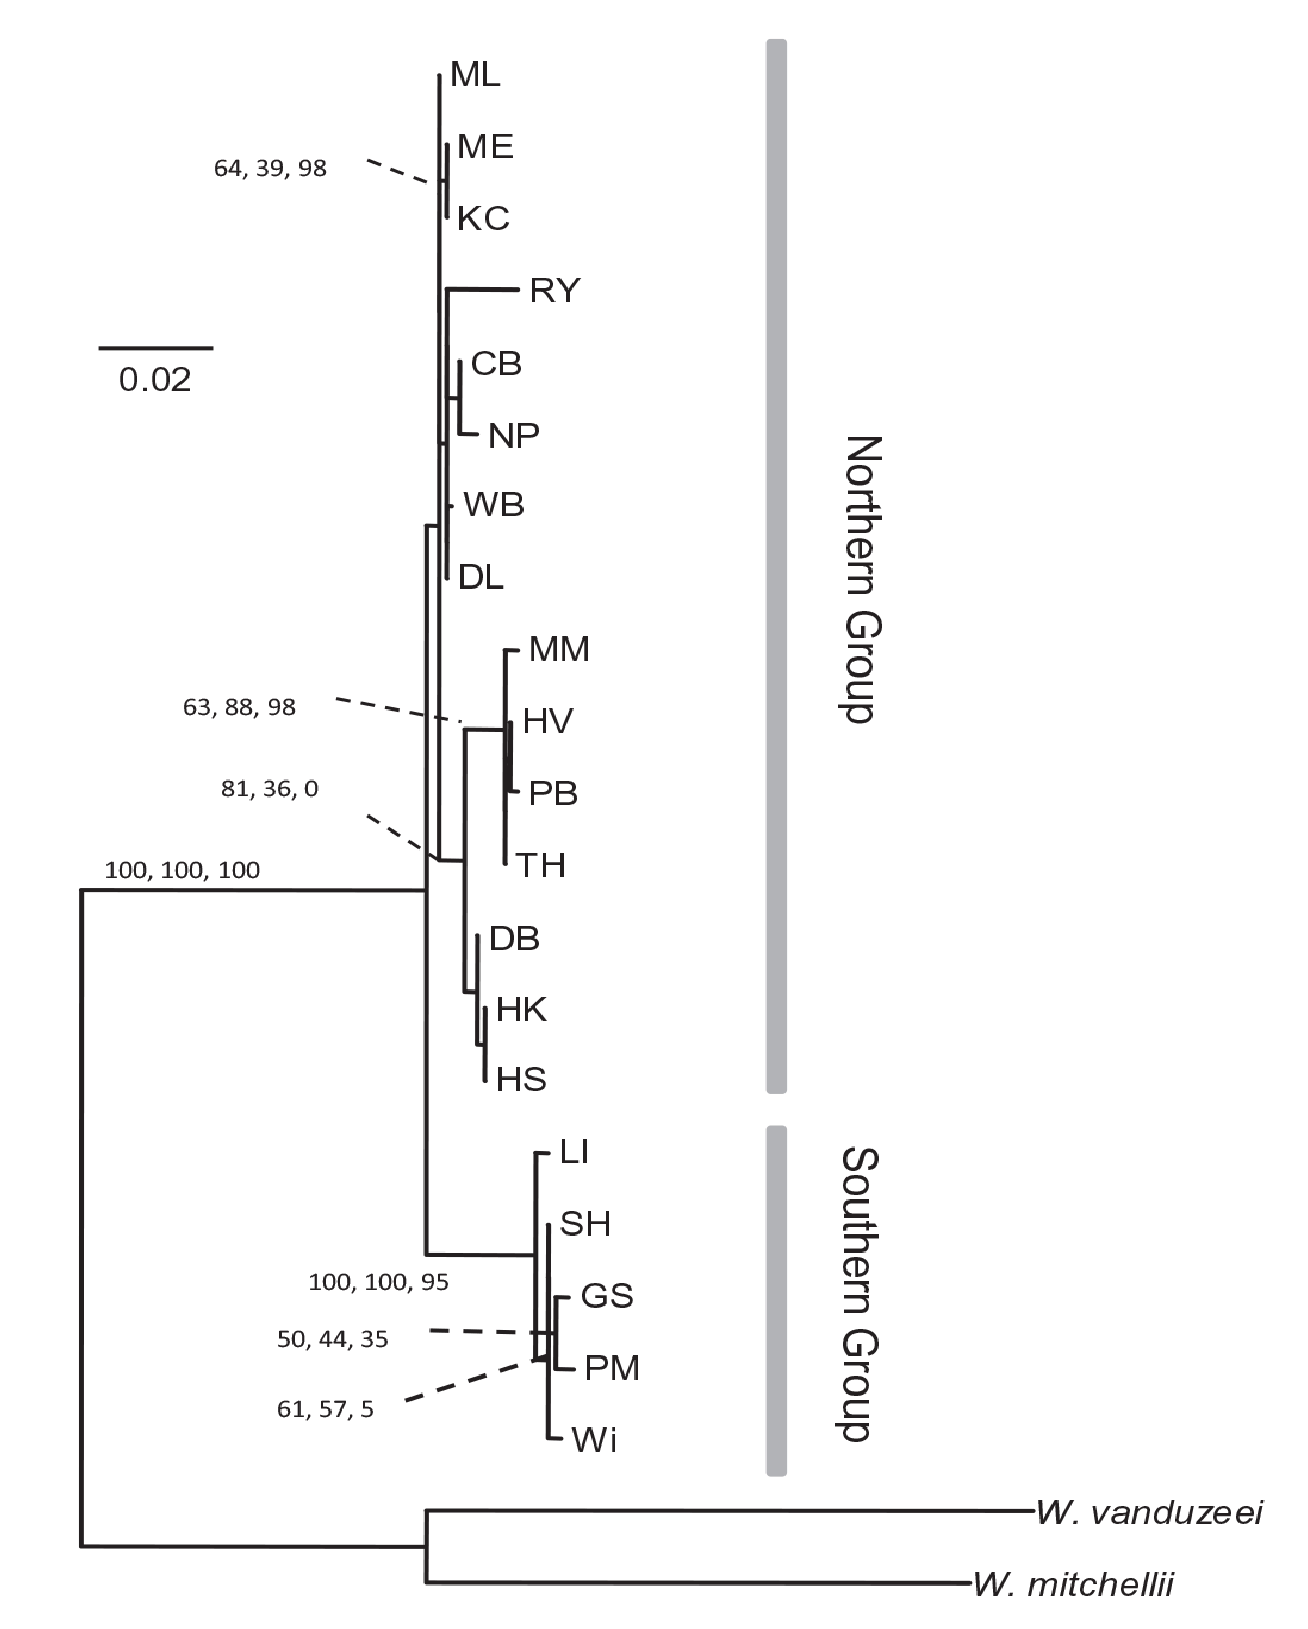
\includegraphics[height=0.9\textheight]{wyeomyia-COI.eps}
\end{center}
}

\myslide{
\heading{{\it Wyeomyia smithii\/} (RAD-seq)}
\begin{center}
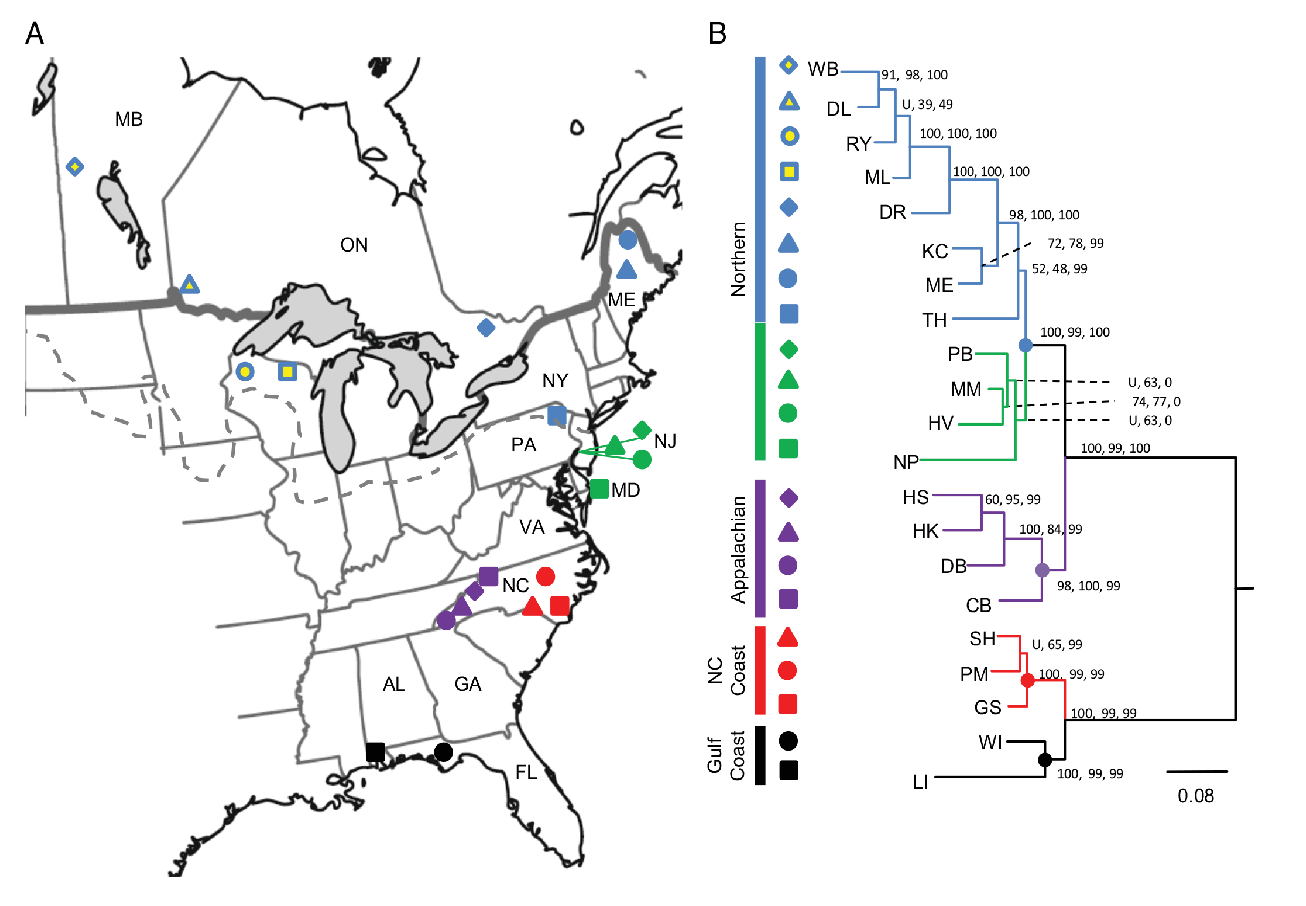
\includegraphics[height=0.9\textheight]{wyeomyia-RAD.eps}
\end{center}
}

\myslide{
\heading{Homozygous site}
\[
P(n_1,n_2,n_3,n_4|\mbox{homozygous A},\epsilon)
=
{n \choose n_1}(1-\epsilon)^{n_1}\epsilon^{n-n_1}
\]
\vfill
\[
P(n_1,n_2,n_3,n_4|\mbox{homozygous},\epsilon)
=
\sum_{i=1}^4 \left(\frac{p_i^2}{\sum_{j=1}^4p_j^2}\right) 
{n \choose n_i}(1-\epsilon)^{n_i}\epsilon^{n-n_i}
\]
}

\myslide{
\heading{Heterozygous site}
\begin{eqnarray*}
P(k_1,k_2)
&=&
{n \choose k_1}\left(\frac{1}{2}\right)^{k_1}
               \left(\frac{1}{2}\right)^{k_2}
\\
&=&
{n \choose k_1}\left(\frac{1}{2}\right)^n
\end{eqnarray*}
\vfill
{\footnotesize
\begin{eqnarray*}
P(n_1,n_2,n_3,n_4|x_i,x_j,k_1,k_2) &=& \\
\sum_{l=1}^4\sum_{m=0}^{k_1}{k_1 \choose m}(1-\delta_{il})^m\delta_{il}^{k_1-m}
{k_2 \choose n_i-m}(1-\delta_{jl})^{n_1-m}\delta_{jl}^{k_2-(n_1-m)}
\end{eqnarray*}
}
where 
\[
\delta_{il} = \left\{\begin{array}{ll}
1-\epsilon & \mbox{if } i = l \\
\epsilon & \mbox{if } i \ne l \quad .
\end{array}
\right.
\]

}

\myslide{
\heading{Heterozygous site}
\[
P(n_1,n_2,n_3,n_4|x_i,x_j,\epsilon) =
P(n_1,n_2,n_3,n_4|x_i,x_j,k_1,k_2,\epsilon)P(k_1,k_2) \quad ,
\]
\vfill
{\footnotesize
\[
P(n_1,n_2,n_3,n_4|\mbox{heterozygous},\epsilon)
=
\sum_{i=1}^4\sum_{j\ne i}
\left(\frac{x_ix_j}{1-{\sum_{l=1}^4p_l^2}}\right) P(n_1,n_2,n_3,n_4|x_i,x_j,\epsilon) 
\]
}
}

\myslide{
\heading{Nucleotide diversity}
\[
\pi = \mbox{Probability that a site is heterozygous}
\]
\vfill
{\tiny
\[
P(n_1,n_2,n_3,n_4|\pi,\epsilon)
=
\pi P(n_1,n_2,n_3,n_4|\mbox{heterozygous},\epsilon)
+
(1-\pi)P(n_1,n_2,n_3,n_4|\mbox{homozygous},\epsilon) \quad .
\]
}
\vfill
\[
P(\mbox{data}|\pi,\epsilon) = \prod_{s=1}^S
P(n_1^{(s)},n_2^{(s)},n_3^{(s)},n_4^{(s)}|\pi,\epsilon) \quad ,
\]
}

\myslide{
\begin{center}
\begin{tabular}{lccc}
\hline\hline
Taxon & $4N_e\mu$ & $4N_e\mu$ (low coverage) & $\epsilon$ \\
\hline
{\it Cionia intestinalis} & 0.0111 & 0.012 & 0.00113 \\
{\it Daphnia pulex} & 0.0011 & 0.0012 & 0.00121 \\
\hline
\end{tabular}
\end{center}
}

\myslide{
\heading{PCA of population structure}
\begin{center}
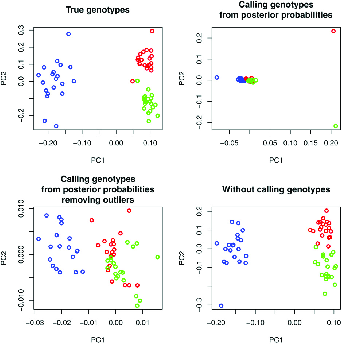
\includegraphics[height=0.8\textheight]{fumagalli-PCA.eps}
\end{center}
}

\myslide{
\heading{Population genomics in Great Britain}

Data
\begin{itemize}

\item 2039 individuals with four grandparents born within 80km of one
  another, effectively studying alleles sampled from grandparents
  (ca. 1885). 

\item 6209 samples from 10 countries in continental Europe.

\item Autosomal SNPs genotyped in both samples~(ca. 500K). 

\end{itemize}
\vfill
Results
\begin{itemize}

\item Average pairwise $F_{ST}$: 0.0007

\item Maximum pairwise $F_{ST}$: 0.003

\end{itemize}
}

\myslide{
\heading{Population genomics in Great Britain}

\begin{center}
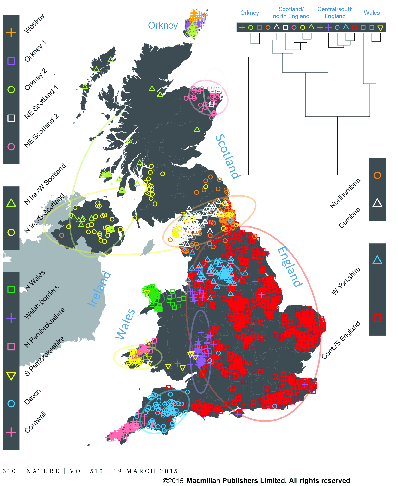
\includegraphics[height=0.9\textheight]{fine-structure-britain.eps}
\end{center}
}

\myslide{
\heading{Population genomics in Great Britain}

\begin{center}
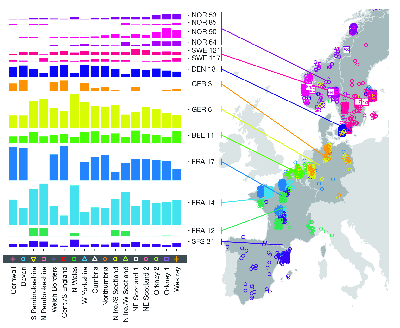
\includegraphics[height=0.9\textheight]{UK-Europe.eps}
\end{center}
}

\end{document}

